\documentclass[letterpaper]{jdf}
\addbibresource{project-references.bib}
\usepackage{minted}

\author{Kyle King}
\email{kking303@gatech.edu}
\title{CS-6750 Summer 2022 Project}

\begin{document}

\maketitle

\begin{abstract}
    Many developers utilize some form of "dotfile" management where they use tools to backup, version control, and/or synchronize text-based configuration files across computers. One popular tool, \emph{yadm: Yet Another Dotfile Manager}, has many strengths, but has a few usability issues as identified in a Think-Aloud interview and two surveys. Based on the need finding insights and a heuristic analysis, a Terminal User Interface was proposed as a potential way to resolve the most prominent usability issues. Additional iterations through the User Centered Design process are necessary and an Evaluation protocol is proposed for future work.
\end{abstract}

\section{Introduction}
Many developers spend time personalizing their computers, and over the years, may accrue an extensive set of custom configuration for everything from basic Shell PATH manipulations to extremely personalized vim configurations \citep{Hahn2022}. There are dozens of ways for tracking, syncing, and generally managing these files, which are broadly known as "dotfiles" because of the Linux convention of a leading period \citep{Borkiewicz2019}. Based on the list of top tools on \href{https://dotfiles.github.io/utilities/}{https://dotfiles.github.io/utilities/} \citep{DotfileChoices}, I reviewed the top three projects based on star count and selected \emph{yadm: Yet Another Dotfile Manager} (Stars: 3540) \citep{TheYadm}. I chose \emph{yadm} over chezmoi, because chezmoi requires separate steps to edit and apply changes, while with \emph{yadm}, the files are edited directly \citep{ChezmoiTable}. When compared to DotBot \citep{Athalye2014} or Stow \citep{Invergo2012}, \emph{yadm} appeared to be more opinionated in a way that may be better suited for beginners who will need to make fewer decisions.

\emph{yadm} can be found \href{https://github.com/TheLocehiliosan/yadm}{on Github} and has a \href{https://yadm.io/docs/overview}{documentation website}. To start, users can either manually install using the command below \citep{YadmQuickStart} or \href{https://yadm.io/docs/install}{seek out an installer for their operating system}. Make sure that the \emph{yadm} executable is present on your PATH and that git is installed.

% <------------ Keep on same page ------------>
\newpage
\begin{minted}[frame=single,
               breakanywhere=true,
               fontsize=\small,
               tabsize=4]{sh}
# As a generic way of installing for most Mac and Linux shells, run:
curl -fLo /usr/local/bin/yadm https://github.com/TheLocehiliosan/yadm/raw/master/yadm \
    && chmod a+x /usr/local/bin/yadm

# Quick Start

# Initialize
yadm init
# Add the first file (example file)
touch ~/.test-file
yadm add ~/.test-file
# Begin tracking changes
yadm commit
# Now edit (or remove the file) and see the difference
rm ~/.test-file
yadm status

# From here, there are plenty of more advanced features, such as templating,
#   encryption, and files that are OS-specific
# For examples, take a look at: https://yadm.io/docs/examples#
\end{minted}

\section{Initial Needfinding}

\subsection{Initial Needfinding: Think Aloud}
In order to gain a better understanding of user tasks and needs, I will conduct a single think-aloud interview. The participant will talk through the task of cloning a repository; make local edits, commit, and push; and the task of pulling new changes.

The user was a Senior Software Engineer who was comfortable with the command line. After resolving a few issues installing the necessary package and \emph{transcrypt} dependency, the participant attempted to clone the shared dotfiles repository, but immediately ran into an issue with git for differences with their local files. Before and after cloning, the participant was unsure what would happen to these files. In particular, the git labels were not necessarily clear for which file was from where. To resolve the issue, the participant did not know the necessary git commands by memory, but could quickly reference them from documentation or by web search. Making changes, pushing, and then pulling were straightforward.

\subsection{Needfinding: Survey 1}
Based on the Think Aloud, I developed a survey to gather feedback from a wider audience and understand the generalizability of the initial insights. To target the right users, the survey was shared with the CS-6750 class asking for participants who were at least partially familiar with dotfiles and on Reddit in \emph{r/dotfiles}. After ten days, the survey received eighteen responses and the raw results are captured in Appendix \ref{appendix:survey_1_results}.

\subsubsubsection{Who are the users?} The participants are highly technical and frequently use a terminal every day (Figure \ref{fig:survey_count_terminal}), they have multiple synced computers (Figure \ref{fig:survey_count_computers}), and they use a wide breadth of tools for managing dotfiles (Figure \ref{fig:survey_which_tools}). They are predominantly Associate, Senior, Principal, or Staff Software Engineers, but also include two Technical Leads, a Cloud Security Engineer, an Analyst, and a Data Scientist.

\begin{jdffigure}
\includegraphics[height=8cm]{./Figures/bar-Terminal-Use-Frequency.png}
\captionof{figure}{How frequently do you use a terminal, such as Windows Command Prompt or Mac Terminal?}\label{fig:survey_count_terminal}
\end{jdffigure}

\begin{jdffigure}
\includegraphics[height=8cm]{./Figures/bar-Count-of-Computers.png}
\captionof{figure}{On how many computers (virtual or physical) do you currently have your dotfiles?}\label{fig:survey_count_computers}
\end{jdffigure}

\begin{jdffigure}
\includegraphics[height=12cm]{./Figures/multi-select-Tools-for-Management.png}
\captionof{figure}{Which software application(s) do you currently use to for managing "dotfiles" (Desktop configuration files, such as ".bashrc" or "~/.config/nvim/init.vim")?}\label{fig:survey_which_tools}
\end{jdffigure}

\subsubsubsection{Where are the users?} The participants are managing dotfiles either at work and/or on their own time.

\subsubsubsection{What is the context of the task?} The participants are working with coworkers to sync configurations and/or managing their individual dotfiles separately.

\subsubsubsection{What are their goals?} The participants reported variations of the need to have a "consistent user experience across my various machines" and to manage changes to complex configuration files.

\subsubsubsection{What do they need?} Different participants had competing needs. Some valued privacy and security, while others were open to public files at the benefit of ease of use. One participant reported the need to sync dotfiles offline through a flashdrive rather than on hosted services, like Github. Multiple participants indicated that they wanted to use a tool they were familiar with and didn't want to lean something new. They also indicated that they didn't always know what they need from a dotfile manager until they started tracking files and developed custom scripts that fit their immediate needs.

\subsubsubsection{What are their tasks?} Participant tasks and subtasks include:

\begin{itemize}
	\item Initialize, add, and remove files
	\item Store the files in version control and resolve differences
	\item Encrypt and conceal secrets stored in the configuration files
	\item Sync files across computers and account for machine-to-machine differences
	\item Manage installed software related to synced dotfiles
	\item Coordinate and share snippets with team members (which is still done largely through Slack, Wikis, and other manual processes)
	\item Forking and nitpicking snippets from public dotfiles
	\item Separate work and personal configurations
\end{itemize}

\subsection{Targeted Needfinding: Survey 2}
Based on the first survey and initial Think Aloud, there were a few areas that could be explored with the redesign. To gain quantitative insight and help further focus the prototype, I created a second survey of the design changes being considered and sent the survey to a few individuals who had completed Survey 1.

The survey had only two responses and the entire results are available in Appendix \ref{appendix:targeted_needfinding}. The first participant identified a few potential bugs that were difficult to recover from, which identified the need for potentially better Tolerance and Constraints in the design since software bugs in open source software are inevitable. Additionally, a theme that emerged was that \emph{yadm} was difficult to comprehend and debug when pulling changes and managing templates. Two notable quotes from the survey are highlighted below:

\begin{quotation}
	"I would have yadm be more verbose about what it was doing under the hood. It's a great tool, but feels a little too magicky for me."
\end{quotation}

\begin{quotation}
	"Can be confusing when first setting up to align shared dotfiles with existing local - `git reset --hard HEAD` seems too forceful. Templates break too easily / don't error when they should."
\end{quotation}

One of the participants also highlighted a feature from \emph{yadm} and almost all dotfile management tools that is currently missing:

\begin{quotation}
	"While syncing dot files is fantastic among collaborators at any project, I would prefer if the entire files didn't have to be synced. A selective sync/composability would be the killer feature for me."
\end{quotation}

\section{Heuristic Evaluation}

\subsection{yadm: Heuristic Strengths}
\emph{yadm} meets five of the course's superset of Human-Centered Design  Heuristics, which include \emph{Simplicity}, \emph{Comfort}, \emph{Documentation}, \emph{Consistency}, \emph{Mapping}, and \emph{Flexibility}.

\subsubsubsection{Simplicity} \emph{yadm} meets the usability heuristic of simplicity by keeping all files where they natively. Other tools may have more complicated symlinking or multi-step edit and apply workflows, while \emph{yadm} doesn't change the user's existing filesystem. Having the files located in their normal locations means that developers can make changes and see the results immediately maintaining a fast \emph{feedback} cycle on changes.

\subsubsubsection{Comfort} \emph{yadm} provides an entirely textual interface that utilizes the same user peripherals as any other computer application. A user can interact with \emph{yadm} with their existing inputs, such a joystick-based text entry interface or an ergonomic keyboard. Additionally, \emph{yadm} uses short subcommands and avoids unusual symbols, which addresses both \emph{comfort} and \emph{ease}.

\subsubsubsection{Documentation} \emph{yadm} provides documentation in several ways. On the \emph{yadm} website, there are examples for getting started, an API reference, and documentation on advanced features. From the CLI, \emph{yadm --help} or \emph{man yadm} provide offline documentation. Lastly, the \emph{yadm} source code is public and includes comments that are contextual relevant when a developer seeks to understand the implementation.

\subsubsubsection{Consistency} The primary \emph{yadm} user is a developer who is comfortable working with command line (CLI) tools. As such, \emph{yadm} follows standard CLI conventions, such as providing subcommands (\emph{yadm init}) and utilizing flags (\emph{yadm --help}). For version control, \emph{yadm} wraps the git CLI, which means that all commands from git are available in \emph{yadm}, with only minor modification where needed. Each git subcommand through \emph{yadm} provides consistent functionality, such as how \emph{yadm clone} "clones" the hosted repository in the default location for \emph{yadm}.

\subsubsubsection{Mapping} Being a text-based command line interface, \emph{yadm} can only implement mapping by the vocabulary used for the subcommands and flags. All twelve of the \emph{yadm-specific} subcommands are closely related to the associated task (\emph{init, clone, config, list, alt, bootstrap, encrypt, decrypt, perms, enter, git-crypt, transcrypt}). \emph{yadm encrypt} encrypts the specified file, which can be used with the inverse, \emph{yadm decrypt}. In another case, \emph{yadm transcrypt} is used to interact with the external \emph{transcrypt} library.

\subsubsubsection{Flexibility} \emph{yadm} does not explicitly provide flexibility for user configuration, but flexibility is inherent in the shell environment where \emph{yadm} is used and for the git CLI utilized by \emph{yadm}. Users can choose to add shell functions or aliases then sync those with \emph{yadm} to make running frequent commands easier and more efficient. \emph{yadm} provides information so that tab completion is possible where users can start typing, then press tab to finish entry of the command.

\subsection{yadm: Heuristic Weaknesses}
While \emph{yadm} has many strengths, there are a few heuristics areas where \emph{yadm} could be improved.

\subsubsubsection{Discoverability} \emph{yadm} has sufficient documentation on their website, CLI, and source code as described as a strength, but a developer must reference these resources to learn what functionality is available and how to use \emph{yadm}. The need to reference this documentation contributes to a steeper learning curve and can make learning how to use \emph{yadm} more difficult, but since the documentation is available, this can be considered a PASS with Difficulty heuristic finding and still a weakness.

\subsubsubsection{Gulf of Evaluation} For users who sync changes across computers or between users, a user's set of local files managed by \emph{yadm} may frequently become out of sync with the hosted versions. Typically this can be resolved with \emph{pull} which will update all files in-place, but any local changes may create conflicts that require manual resolution. This is currently an area where \emph{yadm} doesn't provide any specific tooling and relies on existing git tools, which are typically configured for normal git repos and not this edge case. This application state can be replicated with the steps shown in Appendix \ref{appendix:yadm_pull_deletes}.

Based on git configuration, the resulting git status may appear to show that the file was deleted, which could be very confusing to a user who is now unsure of what to do. Additionally, the deleted file is staged, but the local file is still present as verified by running \emph{cat}. A user might reasonably expect to either see the diff or have an error raised that the clone could not be done safely. This particular usability issue likely arose from \emph{Expert Blindspot} where managing state before cloning or recovery from this state is something avoided subconsciously.

\subsubsubsection{Tolerance} Actions in git can sometimes be undone, but that can be a complicated process and has a high risk of  accidentally losing local changes if not careful or losing track of what had changed. However, the more pressing issue is the sensitivity of the configuration files controlled by \emph{yadm}. In situations like the one described above, git can add text to the file indicating a diff while working on a rebase. If the configuration file is loaded at the same time or used by other applications, the syntax error could have substantial consequences and potentially lock out the user from their computer. While this corner case is unlikely, the risk is high and inherently a side effect of the design for \emph{Simplicity}.

\section{Interface Redesign}
The interface redesign is shown as a series of sequential mockups. The first card shows the context of running on MacOS while the rest focus only on the Terminal emulator which is generic to any supported OS. The tool can be run on any Linux-based system including \emph{Windows Subsystem for Linux}. Importantly, this version of the prototype is read-only and changes must be made in the user-specified Editor.

\begin{jdffigure}
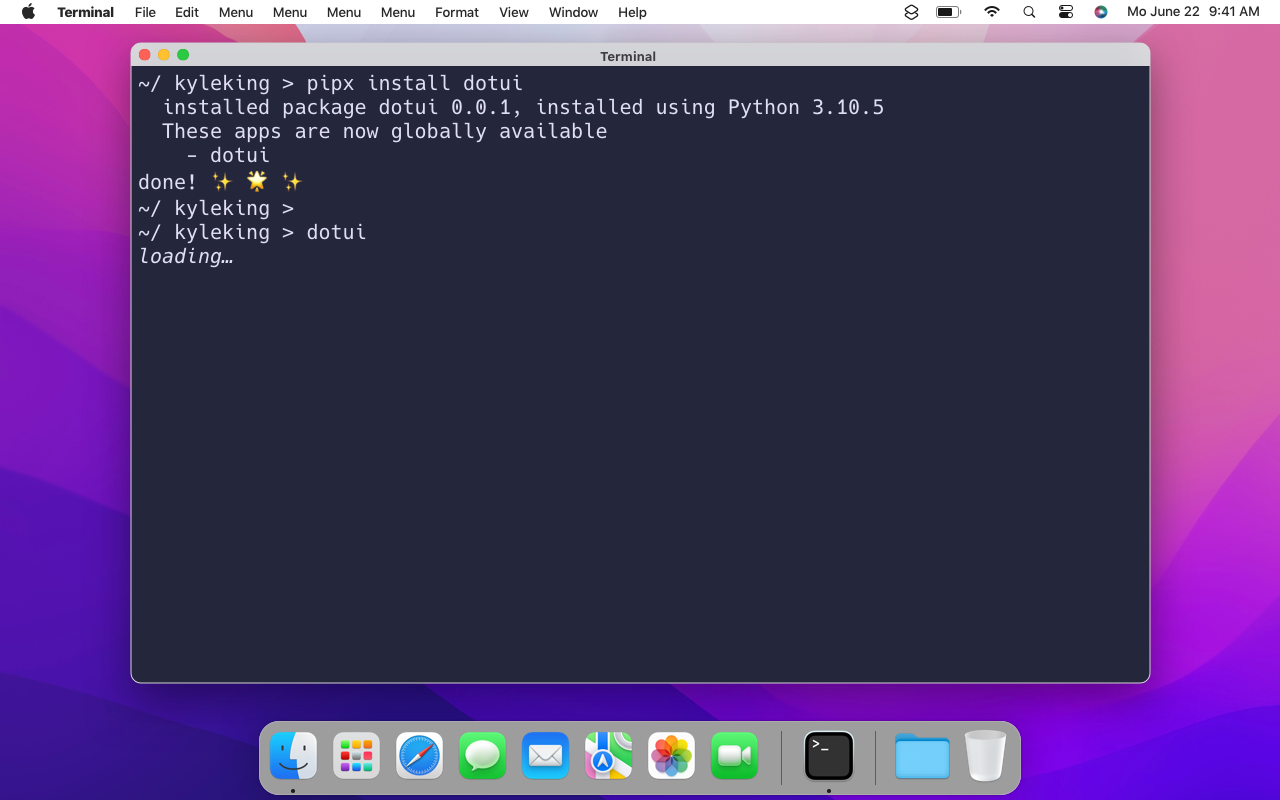
\includegraphics{./Prototype/Card01-Install.png}
\captionof{figure}{Card01}\label{fig:Card01}
\end{jdffigure}

\begin{jdffigure}
\makebox[\textwidth]{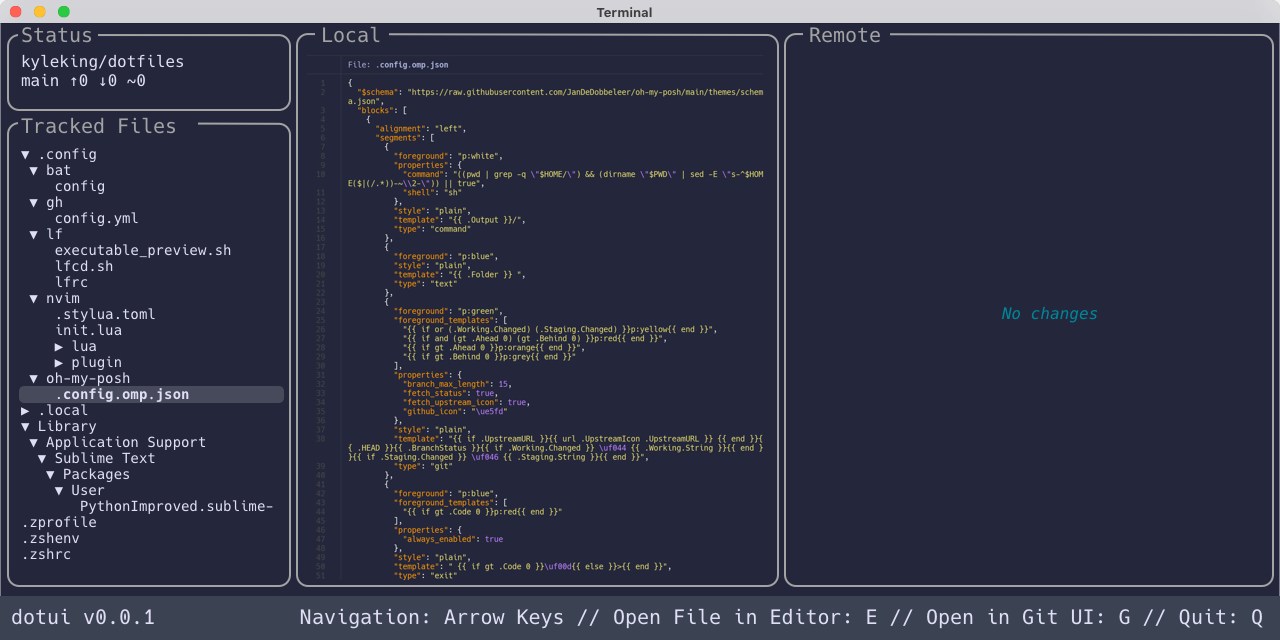
\includegraphics[width=20cm]{./Prototype/Card02-NoDiff.png}}
\captionof{figure}{Card02}\label{fig:Card02}
\end{jdffigure}

\begin{jdffigure}
\makebox[\textwidth]{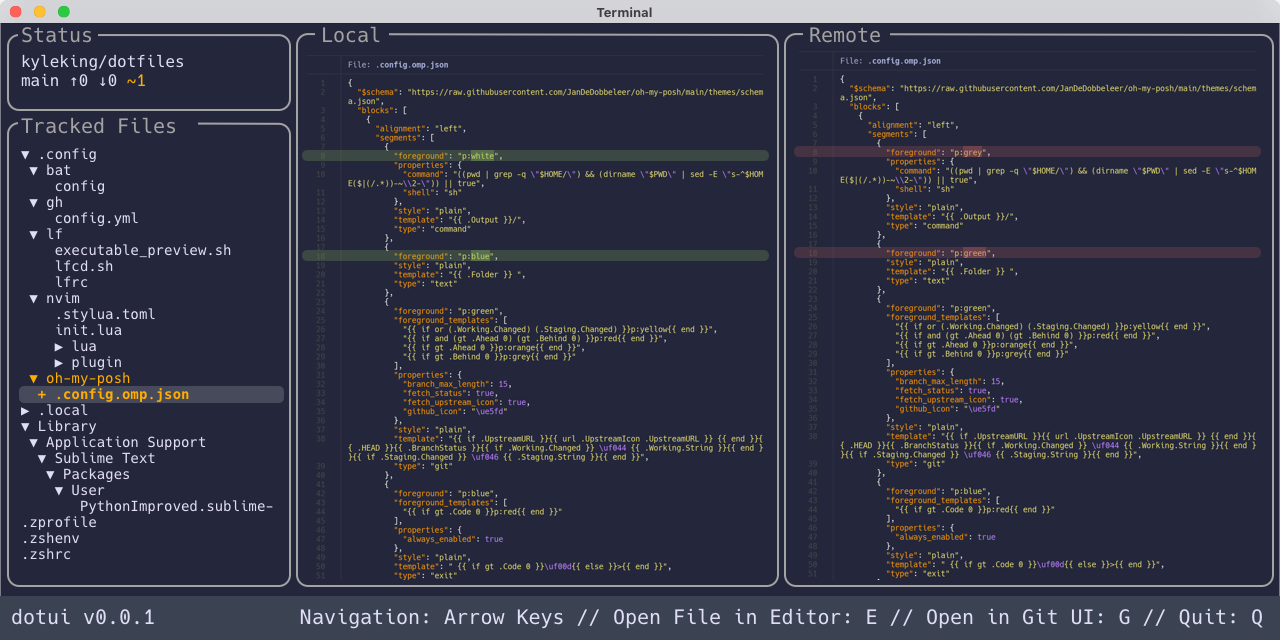
\includegraphics[width=20cm]{./Prototype/Card03-Diff.png}}
\captionof{figure}{Card03}\label{fig:Card03}
\end{jdffigure}

\begin{jdffigure}
\makebox[\textwidth]{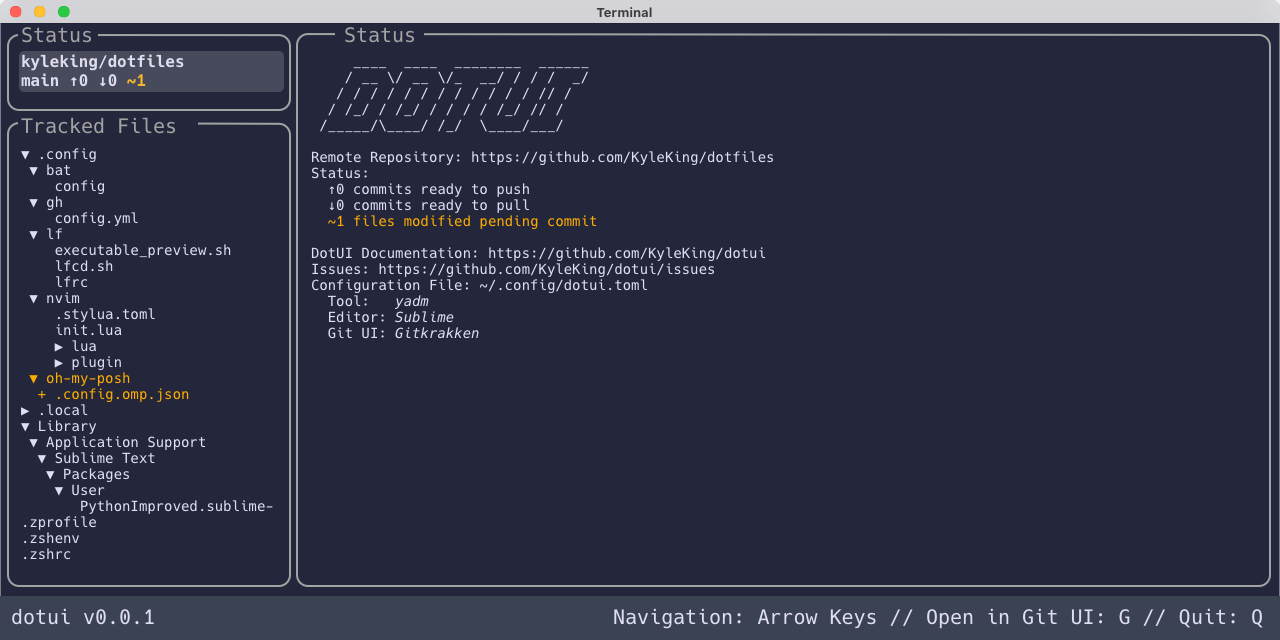
\includegraphics[width=20cm]{./Prototype/Card04-Status.png}}
\captionof{figure}{Card04}\label{fig:Card04}
\end{jdffigure}

\begin{jdffigure}
\makebox[\textwidth]{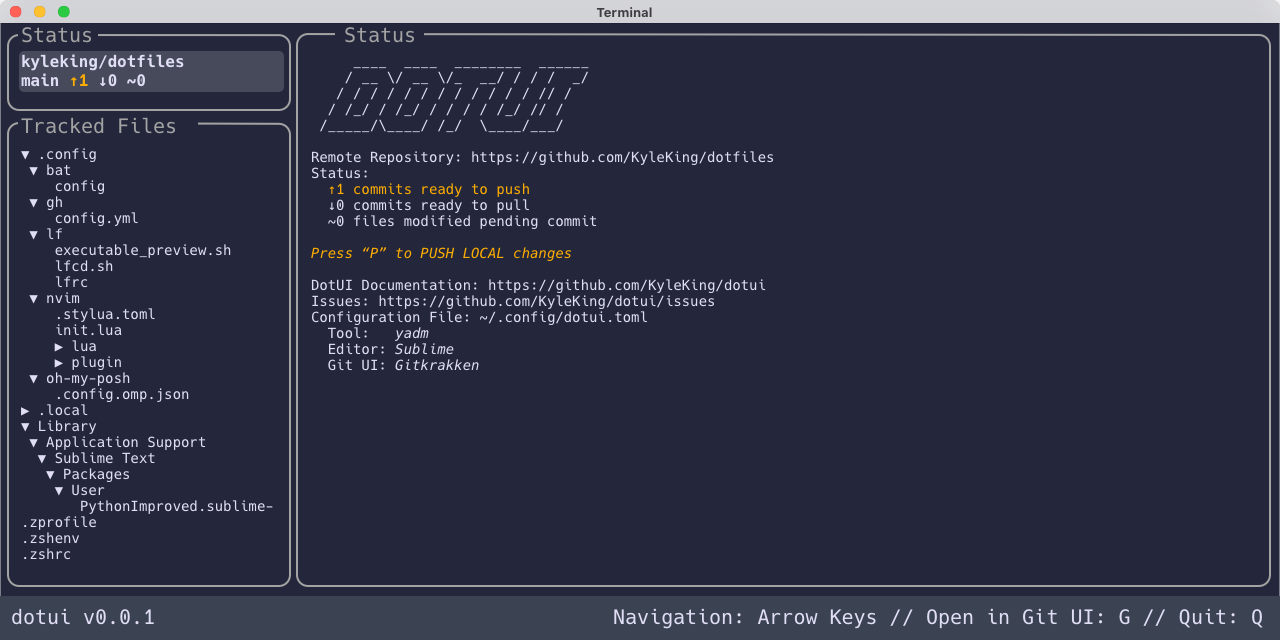
\includegraphics[width=20cm]{./Prototype/Card05-Push.png}}
\captionof{figure}{Card05}\label{fig:Card05}
\end{jdffigure}

\begin{jdffigure}
\makebox[\textwidth]{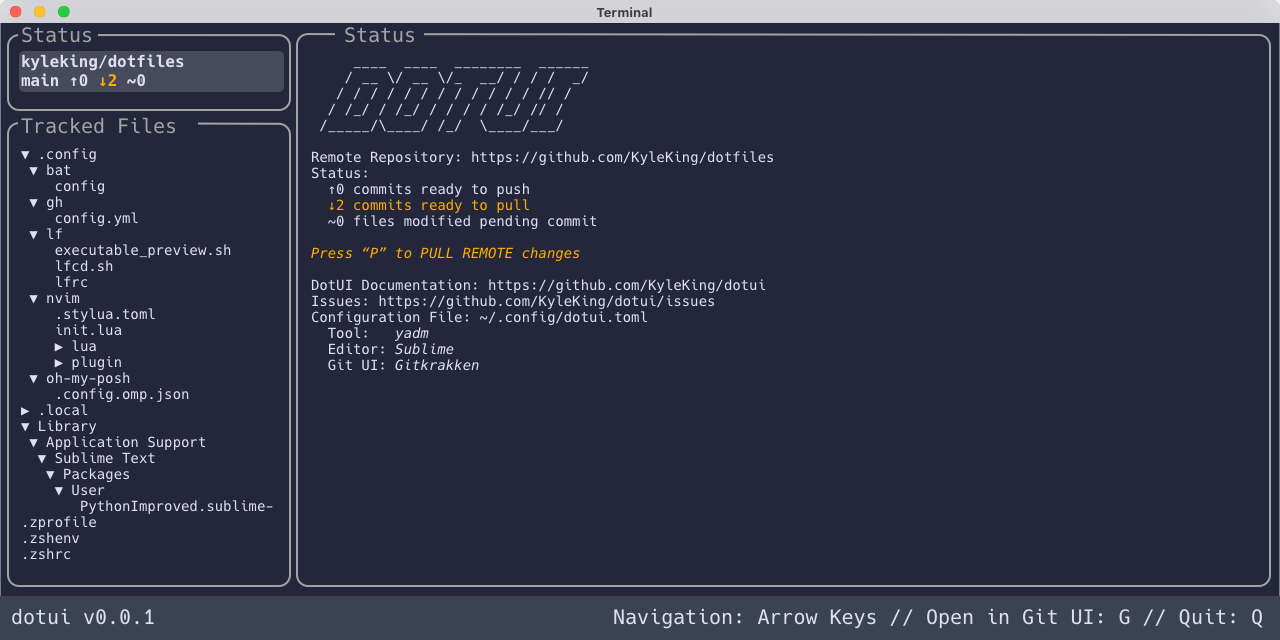
\includegraphics[width=20cm]{./Prototype/Card06-Pull.png}}
\captionof{figure}{Card06}\label{fig:Card06}
\end{jdffigure}

\begin{jdffigure}
\makebox[\textwidth]{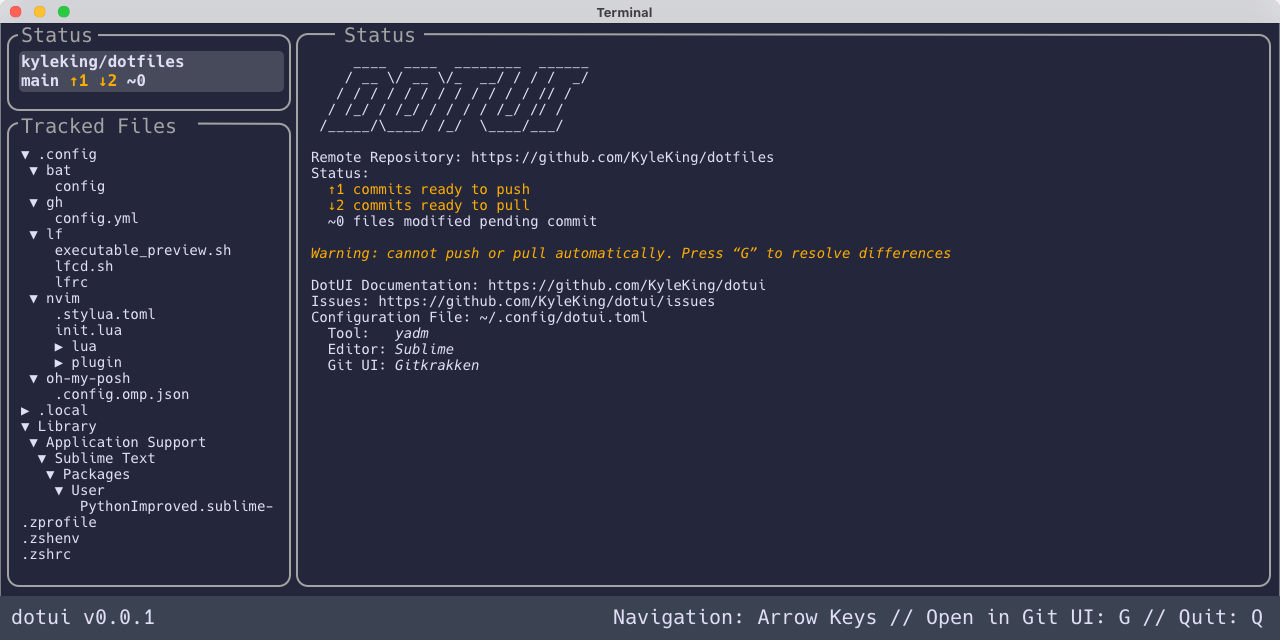
\includegraphics[width=20cm]{./Prototype/Card07-Conflict.png}}
\captionof{figure}{Card07}\label{fig:Card07}
\end{jdffigure}

\subsubsubsection{Note} Figure \ref{fig:Card08} is shown with a proposed \emph{v0.0.2} change where a new section, \emph{Templates}, is added. If the previous cards were to be updated, the \emph{Templates} section would be shown in the bottom left with a shorter \emph{Tracked Files} section and scrollbar. Like the other cards, the bottom help text is context-dependent and updates based on the main panel view.

\begin{jdffigure}
\makebox[\textwidth]{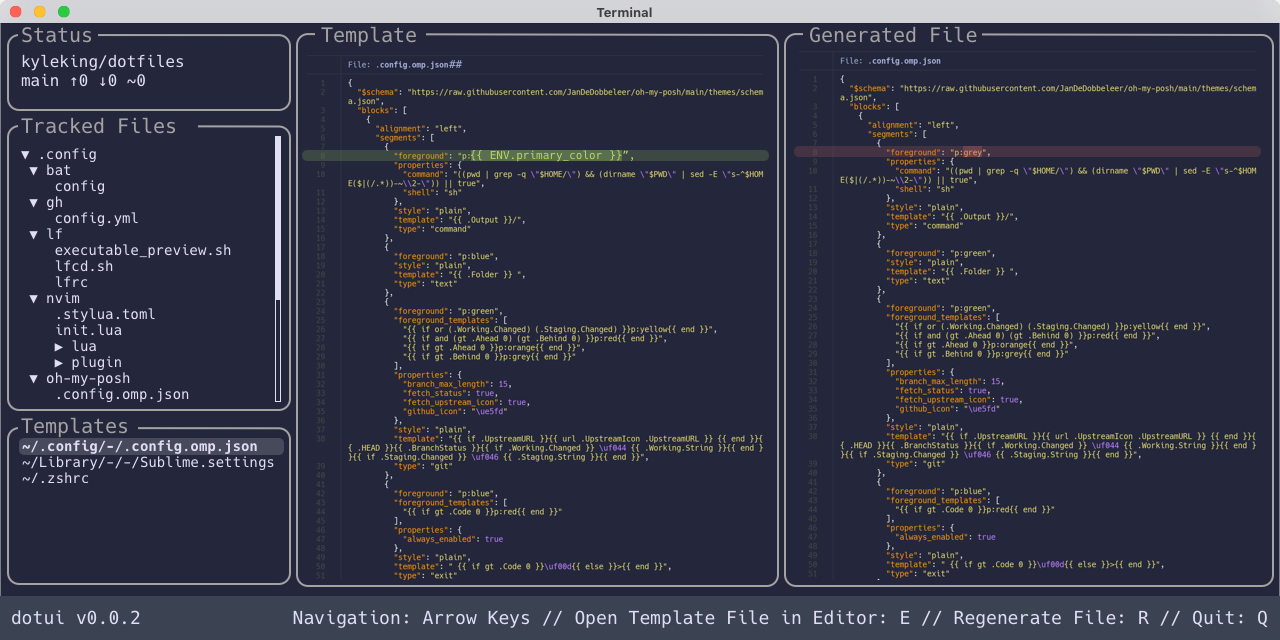
\includegraphics[width=20cm]{./Prototype/Card08-Template.png}}
\captionof{figure}{Card08}\label{fig:Card08}
\end{jdffigure}

\section{Interface Justification}
The interface was redesigned with a focus on user tasks, such as better external tool integration; improving discoverability; reducing the cognitive load; and improving constraints to avoid errors. Further, the prototype \emph{dotui} interface is not mutually exclusive with the \emph{yadm} CLI and both will likely continued to be used, but most tasks can be done from the TUI or user-specified applications rather than in the CLI directly.

\subsubsubsection{Reduce Cognitive Load} Based on issues raised during the needfinding stage, a TUI became a likely candidate to improve usability. Providing a TUI around the \emph{yadm} interface means that users have a visually persistent and live-updating list of all tracked files and git status, which reduces the \emph{Cognitive Load} for users. Users currently need to re-run the \emph{yadm list} or \emph{yadm status} commands to see which are tracked and what has changed respectively, but that can now be seen in one place without the need to scroll back through the terminal buffer. Further, the TUI polls the remote and local changes on a reasonable interval, so that the user has all of the information in one place and doesn't need to remember the state.

\subsubsubsection{Flexibility} A major theme in the first survey was that users wanted to use tools that were familiar to them, which was a major motivation for why they created their own scripts or used a combination of tools they were familiar with. The redesign took this into account by proposing a design that is not tool-specific and external tools are prioritized.

The initial prototype would support only \emph{yadm}, but the implementation could utilize plugins and a Model-View-Presenter architecture that would facilitate support of additional tools in the future. The TUI Views were designed around general tasks that are commonly found in dotfile management tools regardless if the tool is a custom script or a competing project. Users can contribute plugins that meet the prescribed interface to return the list of tracked files, list of templates and generated files, and other details about status, which can then be polled and displayed in the TUI. The prototype does make some assumptions about the use of git, but that was the version control tool of choice and something that could be later refactored to be configurable.

Throughout the \emph{dotui} prototype, there are reminders of the keyboard shortcuts that directly open a user-specified external tool. For files ("E"), the specified Editor is opened, which could be used with any application from VSCode to TextEdit or which could fallback to the system default (i.e. \emph{open ...} on MacOS). For the bare git directory ("G"), the user-specified editor can be opened, which is something that requires advanced knowledge now, but several editors could be supported by default.

Overall, the core \emph{Flexibility} heuristic analyzed as a strength of the \emph{yadm} CLI is extended and improved upon with this prototype. The user-configurable integrations with external tools and ultimately allowing \emph{yadm} to be optional leads to much greater flexibility.

\subsubsubsection{Simplicity, Comfort, and Documentation} The prototype still relies on \emph{yadm} and doesn't make any fundamental changes to the feature-set. Users will still need to access the \emph{Documentation} for certain advanced features and the \emph{Simplicity} of the fundamental design decision for a bare git repository is unchanged. Additionally, the TUI continues to be entirely keyboard driven so that the user's preferred inputs will continue to work and the number of commands were kept to a minimum.

\subsubsubsection{Mapping} The selected keyboard shortcuts for the prototype attempt to reasonable map the shortcut to the name by picking appropriate letters. For example, "G" for Git UI, "E" for Editor, "P" for Push and Pull (contextually aware), and "Q" for Quit. Additionally, icons and scrollbars are used where appropriate.

\subsubsubsection{Consistency} The prototype borrows common design elements from general TUIs and comparable Git UIs to make for a consistent user experience across similar tools. The core navigation is managed arrow keys, which is a common interaction method for most TUIs and would be intuitive for most users. When there is a diff from version control the prototype is \emph{externally consistent} by placing the local version on the left. The prototype is \emph{internally consistent} between the diff view and the template and generated file pair view because in both, the local tracked file is on the left.

\subsubsubsection{Discoverability} One of the first partial weaknesses identified in the heuristic evaluation, was that the most relevant \emph{yadm} features were not readily available. With the redesign, the core feature set used for most interactions is now made more clear while there is no change to the more complex features. The TUI doesn't need any separate documentation because it is either self-explanatory based on the user's experience with similar tools or clearly labeled in the help bar along the bottom.

\subsubsubsection{Gulf of Evaluation, Constraints, and Tolerance} The major issue with \emph{yadm's} current design is that errors are very difficult to recover from. This is not easy to address, but there are design changes that can help. The prototype makes two core changes to address this. First, the interface polls for updates so that the current upstream and local state are known at all times that TUI is open. Secondly, when the local and remote states diverge in a way that would make recovery difficult, the TUI informs the user of the possible issue and directs them to a dedicated Git UI that can more adequately resolve the issue. Now, when opening \emph{dotui}, the application launches to the "Status" view where the actionable Pull, Push, or resolve-manually message is shown in plain language.

\subsubsubsection{Future Work} There are several areas where the interface could be improved. One of the areas not addressed with this initial design is the onboarding to an existing \emph{yadm} repository. The initial clone is nearly guaranteed to have some conflicts with the local files, so there could either be changes to \emph{yadm} or a new feature for the prototype to make this step more predictable for the user or generally better align with their mental model.

\subsubsubsection{New Directions} One of the other ideas that was requested during the needfinding stages and explored while brainstorming was a way to compose snippets together from multiple sources. This would require a substantial redesign and is not a trivial problem, but improvements to visualization of templated-files and a better understanding of the needs of this area would help refine possible approaches. There are is at least one product working in this space that was \href{https://github.com/callrbx/meld}{recommended by a participant}.

\section{Qualitative Evaluation Plan}

\subsubsubsection{Prototype Adjustments} The prototypes presented for this assignment are possibly too precise and detailed for the stage of development, but were necessary to meet the constraints of the assignment. For evaluation, the prototypes would be redrawn as abstract wireframes where the color scheme, icons, and font selection are excluded in favor of focusing on core features, such as layout, functionality, and interaction methods. By downgrading the prototype fidelity, participants would be much more likely to critique the design that looks incomplete rather than the current high-fidelity prototype because of Social Desirability bias.

\subsubsubsection{Goals} The goals of the evaluation are to determine if the proposed prototype would be something that the participant would use and to understand the reasoning for either choosing to use the prototype or choosing not to. The qualitative feedback would inform the next iteration of the design cycle as the prototype is refined to best address user tasks, needs, and context.

\subsubsubsection{Interview Logistics} The planned evaluation would be a live demonstration coordinated by two interviews and a single participant at a time. One interviewer will be leading the interview by asking questions, while the second takes notes. At least five participants should be interviewed and participants should have a range of prior experience to best represent the pool of potential users. The participants should be recruited from technical groups on LinkedIn and Reddit. Like Survey 1, each participant should complete a few background questions at the start of the interview by providing their job title, how often they have used a terminal in the past week, and how they manage dotfiles currently. The total interview is expected to take between 15 to 25 minutes.

The interview would be conducted remotely with a web-based whiteboard application that the interviews and participant can see and draw-on.  The video may or may not be recorded based on participant comfort, but screenshots of the whiteboard will be captured when appropriate during the interview and at the end of every interview. The whiteboard would be prepared with one page per Card so that the interviewer can simulate moving between views by changing the visible card. The interview prompt is that the participant is setting up a new laptop at work and needs to figure out how to use the tool to sync local file changes then make a change in \emph{.config.omp.json}.

\begin{enumerate}
	\item "Describe what you see in this screen."
	\item "Is everything on the screen legible?"
	\item "What kind of additional labels or help messages would you add?"
	\item "What next action would take? What button or mouse movement would that involve?"
	\item "What information was missing on this screen?"
	\item "What information was not necessary?"
	\item "What did you dislike about this prototype?"
	\item "What did you like?"
	\item "How would a tool like this fit into your existing workflows?"
\end{enumerate}

The lead interviewer will step through each card and ask the above questions. The interviewer will be sure to reiterate that the user can draw on the prototype and provide feedback visually. The interview should reinforce this by also making small and major changes by drawing on the card in the whiteboard as the open-ended discussion continues. The interviewers should minimize how much time they explain the interface and instead capture notes on any difficult areas that will be addressed in the next design cycle. Once the interview is complete, the participant will complete a survey where they can provide feedback on the interview and rate the prototype on a a five point scale for how likely they are to use it if available and how likely they are to use if their changes were implemented.

\subsubsubsection{Biases} As described above, the primary concern is Social Desirability bias. It will be clear to participants that we had some role in designing the prototype and they may be tempted to provide only non-critical feedback. There are two primary ways the evaluation plan has been designed to minimize this bias. First, the planned questions specifically ask for critical feedback. Second, lower-fidelity card prototypes will be created specifically for these interviews so that participants will feel more empowered to suggest changes. Third, the participant will be asked to quantitatively rate the prototype and their contributions.

To address \emph{Confirmation Bias}, the quantitative post-interview survey will help ensure that the user feedback is properly coded according to the quantitative result. The interview questions are provided to ensure that a base set of qualitative data is captured between subjects, but left open ended because of the stage in the design lifecycle. Finally, the note taker should be someone who has a neutral or different opinion on the topic to the lead interviewer so that the notes best represent the user opinions.

% ------------------------------------------------------------

\section{References}
\printbibliography[heading=none]

\appendix
\section{Appendices}

\subsection{Needfinding Survey Results}\label{appendix:survey_1_results}
Below are the raw results of the survey here. Note that the second question was added after realizing that participants weren't expanding on why they chose Other. Additionally, \emph{Ansible} and \emph{Plain git} were added to the first question after the 10th response based on survey feedback. Although not needed for this paper, there are extensive recent surveys that capture a wider breadth of the tools developers use \citep{Walladge2017}. There is also a survey that could be useful conducted for \emph{Textualize} \citep{McGugan2022}.

\begin{jdffigure}
\includegraphics[height=10cm]{./Figures/wordcloud.png}
\captionof{figure}{Word Cloud of selected Qualitative responses. Turned out to be not as useful as expected. Removed words include: "dotfile dotfiles file files yes sure nope n/a na via"}\label{fig:survey_survey_words}
\end{jdffigure}

\begin{itemize}
    \item Which software application(s) do you currently use to for managing "dotfiles" (Desktop configuration files, such as ".bashrc" or "~/.config/nvim/init.vim")?
    \begin{enumerate}
        \item Custom scripts
        \item yadm
        \item Custom scripts;Mac Time Machine or other computer-wide backup and restore software
        \item Other
        \item Other
        \item yadm;Dropbox
        \item Other
        \item GNU Stow;Custom scripts
        \item Custom scripts
        \item Other
        \item Other
        \item Custom scripts;Other
        \item GNU Stow;Other
        \item Plain git
        \item Plain git;Custom scripts
        \item Dropbox;Plain git;Custom scripts
        \item Plain git;Custom scripts
        \item Other
    \end{enumerate}
    \item If you selected “Other” or “Custom Scripts,” can you elaborate on what tools you use?
    \begin{enumerate}
        \item \emph{Not part of survey when submitted}
        \item \emph{Not part of survey when submitted}
        \item \emph{Not part of survey when submitted}
        \item \emph{Not part of survey when submitted}
        \item \emph{Not part of survey when submitted}
        \item \emph{Not part of survey when submitted}
        \item \emph{Not part of survey when submitted}
        \item \emph{Not part of survey when submitted}
        \item \emph{Not part of survey when submitted}
        \item \emph{Not part of survey when submitted}
        \item \emph{Not part of survey when submitted}
        \item \emph{Not part of survey when submitted}
        \item \emph{Not part of survey when submitted}
        \item \emph{Blank}
        \item Ansible
        \item \emph{Blank}
        \item It's just a bash script that install and configures stuff.
        \item I have a friend who wrote a really cool tool for this called meld. \href{https://lib.rs/crates/meld-config-manager}{https://lib.rs/crates/meld-config-manager}
    \end{enumerate}
    \item What convinced you start managing dotfiles?
    \begin{enumerate}
        \item I wanted a consistent user experience across my various machines.
        \item Kyle making it easy to do.
        \item I've wasted tons of time not being organized without it.
        \item Complexity
        \item New environments
        \item standardizing work and projects
        \item Wanted to share my .zshrc between work and home computers.
        \item my vim configuration got long
        \item career
        \item I have to for maintaining configurations
        \item Consistent configs across many instances I manage
        \item starting to customize my vim \& zsh setup
        \item Ability to use on different computers
        \item I work on a team that requires a consistent .gitignore file to remove bloat from our git repository.
        \item consistency across my systems
        \item No
        \item Save time when changing machines. Avoid losing my dotfiles
        \item Literally writing a rust app to do this
    \end{enumerate}
    \item What is your favorite feature of your preferred dotfile management application (or why did you select it over others)?
    \begin{enumerate}
        \item It's hand rolled and extremely barebones, so I know everything that it does.
        \item Similarity to git, no learning new commands. Manages files in place, no need to move them around.
        \item flexibility and feature extensions
        \item Ansible manages the system too
        \item Git or svn — version controls
        \item Manage your dotfiles across multiple diverse machines, securely.
        \item I just put it in a publicly accessable github repo, then git it from there from whichever machine I'm on.
        \item portability
        \item more control
        \item VSCode because I already use it for code editing
        \item Out of the way and low maintence.
        \item My preferred application for dotfiles management is git. It makes tracking changes easy, and I'm familiar with it already. It does everything I currently need. Syncing is easy via e.g. GitLab, GitHub, and/or own server.
        \item Simplicity, and there wasn't many options around when I started
        \item git is fast, straightforwards, works with the terminal and has a free, online presence, i.e. github.
        \item I can manage the low-level details myself, and understand how to troubleshoot it
        \item Common viewer
        \item I use git and a custom script because it felt easy to do so. I haven't spent much time looking for alternatives.
        \item It can use a flashdrive, a single file, or a remote
    \end{enumerate}
    \item What challenges do you face when managing dotfiles (or what made it difficult to start)?
    \begin{enumerate}
        \item I didn't want to introduce any dependency that I wasn't already using, which limited options.
        \item Differences between machines - esp. work vs personal.
        \item honestly, didn't know what aspects were important. didn't know what I didn't know.
        \item Learning roles
        \item Finding a good place to store them
        \item Manage your dotfiles across multiple diverse machines, securely.
        \item Configuration setting specific to a given machine. I.e. configuration specific to my home PC which won't work elsewhere.
        \item yak shaving
        \item version control
        \item Hard to remember where the files are located
        \item Adding exceptions to set or ignore some config options on remote machines.
        \item Initial setup of git might be slightly confusing (setting up a bare repo, creating a custom `dotfiles` alias wrapper for git). Having non-committed changes makes updates difficult (I have to either commit or stash), but that's actually good design as it makes it hard to destroy unsaved changes. However, it would be technically possible to try to pull and merge if there are no changes in same files as current machine has unsaved changes. But maybe I just don't know how to git properly.
        \item Not much, the most annoying thing is having untracked files for system specific usage
        \item Making sure that other team members get the same file in their system and that they're in sync.
        \item differences across platforms, e.g. Ubuntu vs RHEL vs OSX
        \item System generated filename maintenance
        \item I sometimes forget to keep them in sync. I manually have to separate my personal and work config.
        \item None now, meld is buttery smooth
    \end{enumerate}
    \item If you have used yadm, what do you like or dislike about the tool? (Optionally, if you haven't used yadm, but want to skim the README, feel free to leave feedback here as well)
    \begin{enumerate}
        \item I don't like how much magic it does. I would prefer a solution that was a little more explicit in what it was doing, so people other than the creator could follow along well.
        \item Like: that it uses git commands and files stay in place. Dislike: no way to differentiate between machines.
        \item n/a
        \item \emph{Blank}
        \item First I heard of this
        \item \emph{Blank}
        \item Never used before. From reviewing the README, not sure what it does besides provide some kind of encrypted backup of dotfiles.
        \item * would rather use git directly and only learn one command * os-specific config seems weird; I would rather use branches.
        \item \emph{Blank}
        \item \emph{Blank}
        \item \emph{Blank}
        \item Hmm, haven't used and likely won't. Seems interesting, though. Mostly the same as my current setup, but with the git wrapper already made for me. Encryption seems...interesting. Wouldn't trust it. Most importantly, I'm not willing to install 3rd party packages to every system if I can achieve the functionality without it.
        \item \emph{Blank}
        \item \emph{Blank}
        \item I have not used yadm
        \item \emph{Blank}
        \item It looks quite interesting, I might give it a go eventually.
        \item \emph{Blank}
    \end{enumerate}
    \item Which method(s) do you use for tracking changes and/or syncing?
    \begin{enumerate}
        \item Github, GitLab, BitBucket, or other hosted Git;Local Git
        \item Github, GitLab, BitBucket, or other hosted Git
        \item Github, GitLab, BitBucket, or other hosted Git;Local Git
        \item Github, GitLab, BitBucket, or other hosted Git
        \item Github, GitLab, BitBucket, or other hosted Git;SVN or other non-Git VCS (version control system);rsync
        \item Github, GitLab, BitBucket, or other hosted Git;Local Git;Dropbox
        \item Github, GitLab, BitBucket, or other hosted Git;Local Git
        \item Github, GitLab, BitBucket, or other hosted Git;Local Git
        \item Github, GitLab, BitBucket, or other hosted Git;Local Git
        \item Github, GitLab, BitBucket, or other hosted Git;Other
        \item Github, GitLab, BitBucket, or other hosted Git
        \item Github, GitLab, BitBucket, or other hosted Git;Local Git
        \item Github, GitLab, BitBucket, or other hosted Git
        \item Github, GitLab, BitBucket, or other hosted Git;Local Git
        \item Github, GitLab, BitBucket, or other hosted Git;Local Git
        \item Github, GitLab, BitBucket, or other hosted Git;Local Git;Dropbox
        \item Github, GitLab, BitBucket, or other hosted Git
        \item Other
    \end{enumerate}
    \item If you selected Other, describe what you use here:
    \begin{enumerate}
        \item \emph{Blank}
        \item \emph{Blank}
        \item n/a
        \item Ansible
        \item \emph{Blank}
        \item \emph{Blank}
        \item N/A
        \item \emph{Blank}
        \item \emph{Blank}
        \item Google Drive
        \item A variation of this: \href{https://www.ackama.com/what-we-think/the-best-way-to-store-your-dotfiles-a-bare-git-repository-explained/}{https://www.ackama.com/what-we-think/the-best-way-to-store-your-dotfiles-a-bare-git-repository-explained/}
        \item \emph{Blank}
        \item Tangled emacs org files
        \item \emph{Blank}
        \item \emph{Blank}
        \item \emph{Blank}
        \item \emph{Blank}
        \item \href{https://lib.rs/crates/meld-config-manager}{https://lib.rs/crates/meld-config-manager}
    \end{enumerate}
    \item If you track changes, what do you use to stage changes and resolve conflicts?
    \begin{enumerate}
        \item The git diff/merge tools
        \item \emph{Blank}
        \item n/a
        \item Git
        \item Only my version so I just revert
        \item \emph{Blank}
        \item It's a pretty fast and loose management of dotfiles if I'm being honest. Staging and resolving changes is far more elaborate then what I do. I basically copy-and-paste, whatever I want, and omit/delete what I don't.
        \item git and vim
        \item Git
        \item \emph{Blank}
        \item \emph{Blank}
        \item git, nvim
        \item Git
        \item git terminal
        \item gitlab/vi ;)
        \item GitMerge
        \item I manually resolve them. I don't find myself running into merge conflicts that often though.
        \item \emph{Blank}
    \end{enumerate}
    \item What operating systems do you currently have dotfiles installed on?
    \begin{enumerate}
        \item Mac;Linux
        \item Mac
        \item Mac
        \item Mac;Linux
        \item Mac;Linux
        \item Linux;Windows
        \item Mac;Linux
        \item Mac;Linux;Windows
        \item Mac;Linux;Windows
        \item Mac;Linux;Windows
        \item Mac;Linux;Sync or otherwise run on a Remote SSH Session
        \item Linux;Sync or otherwise run on a Remote SSH Session
        \item Mac;Linux
        \item Mac;Windows
        \item Mac;Linux
        \item Mac;Linux;Windows
        \item Mac;Linux
        \item Mac;Linux
    \end{enumerate}
    \item On how many computers (virtual or physical) do you currently have your dotfiles?
    \begin{enumerate}
        \item 2
        \item 2
        \item 2
        \item 3
        \item 5+
        \item 5+
        \item 3
        \item 4
        \item 2
        \item 2
        \item 5+
        \item 5+
        \item 2
        \item 2
        \item 5+
        \item 4
        \item 3
        \item 5+
    \end{enumerate}
    \item If you sync dotfiles between computers, how do you manage configuration differences between machines?
    \begin{enumerate}
        \item store everything in a remote git repo, then treat it like ay other code base.
        \item Just using yadm on work macs for now so no differences.
        \item don't have to, machines are nearly identical
        \item Ansible variables
        \item Test for release file specific to os
        \item \emph{Blank}
        \item Pretty poorly. I mainly really on using similar machines for portability.
        \item each computer is on it's own branch
        \item I don't
        \item \emph{Blank}
        \item Exceptions in my configs based on the properties of the machine
        \item I have a non-synced, but always sourced (if exists) .device.profile dotfile. It contains any needed differences. Should that not be sufficient, I'd just change dotfiles and perhaps create a new git branch for them.
        \item Load untracked files from the config
        \item Always pull and merge from the main branch on github
        \item Ansible playbooks
        \item \emph{Blank}
        \item \emph{Blank}
        \item \href{https://lib.rs/crates/meld-config-manager}{https://lib.rs/crates/meld-config-manager}
    \end{enumerate}
    \item How do you identify what dotfiles should be managed?
    \begin{enumerate}
        \item Anything where I might have trouble getting it back to it's current state if I lost the file.
        \item For work: files that do not change per-person and otherwise would require individuals to set up.
        \item sub-folders
        \item Whatever apps I’m using
        \item I add to list what I need to remember
        \item in a separate Git directory, usually called ~/.dotfiles
        \item The ones I use most often, i.e. .zshrc and .vimrc
        \item manually
        \item I don't
        \item I have to remember
        \item Any tool I use in multiple locations
        \item manually, I add each file separately if I think it's needed. I usually only add files that I've changed manually.
        \item Software I use and/or customize a lot, if config was complicated, or if I intend to use it on a separate machine
        \item Whatever files are in the repository needs to be managed
        \item I have a base set of them defined by function in Ansible (e.g. git-related, shell-related, etc.)
        \item With their extension and type
        \item Foreseen reusability.
        \item \href{https://lib.rs/crates/meld-config-manager}{https://lib.rs/crates/meld-config-manager}
    \end{enumerate}
    \item How frequently do you use a terminal, such Windows Command Prompt or Mac Terminal?
    \begin{enumerate}
        \item More than 5 times per day
        \item More than 5 times per day
        \item Between 1 and 4 times per day
        \item More than 5 times per day
        \item More than 5 times per day
        \item Between 1 and 4 times per day
        \item More than 5 times per day
        \item More than 5 times per day
        \item A couple of times a week
        \item Between 1 and 4 times per day
        \item More than 5 times per day
        \item More than 5 times per day
        \item More than 5 times per day
        \item More than 5 times per day
        \item More than 5 times per day
        \item Between 1 and 4 times per day
        \item More than 5 times per day
        \item More than 5 times per day
    \end{enumerate}
    \item Have you installed dotfiles from another user for work or personal computer? If so, what did you like or dislike about that process?
    \begin{enumerate}
        \item Yes. I disliked the magic and the process of combining personal dot files with others.
        \item No.
        \item yes, have pulled from github repos
        \item No
        \item No
        \item \emph{Blank}
        \item No, dotfiles are like your favorite hat or hoody. It's not about being the best, it's about having the setup that I want, deficiencies included.
        \item n/a
        \item no
        \item \emph{Blank}
        \item \emph{Blank}
        \item Nope, I don't run random scripts and don't have the need to install anyone's dotfiles
        \item \emph{Blank}
        \item Yes, I like the process of using git since it's straightforward and easy.
        \item Nope
        \item \emph{Blank}
        \item Yes. I often find myself forking their files and nitpicking what I need. I like time savings.
        \item Yes, process is super smooth
    \end{enumerate}
    \item Do you share snippets intended for dotfiles or computer configuration at work? If so, are they shared manually or do you have a tool? Are they in version control and/or synced automatically? Roughly how many people are involved?
    \begin{enumerate}
        \item They are synced through yadm for a team of ~10
        \item Answered from the perspective of work! Not currently managing dotfiles on my personal machine but planning to use yadm.
        \item n/a
        \item Shared via GitHub repo and Gists manually
        \item Teams wiki
        \item \emph{Blank}
        \item Occasionally I will share some dotfile configuration with a coworker if I think they'll benefit. It's a transfer directly between two people.
        \item via slack
        \item no
        \item shared manually
        \item Manually
        \item I'm not sure whether I understood the question. I have an installation script that sets up the `dotfiles` wrapper and clones the git repo. Also installs relevant packages. My dotfile git repo is public.
        \item \emph{Blank}
        \item \emph{Blank}
        \item Typically I use \href{https://onetimesecret.com/}{https://onetimesecret.com/} for one-off things with potentially sensitive data. Otherwise, Ansible (via gitlab)
        \item \emph{Blank}
        \item Yes, sometimes shared in Slack. Some are documented in Confluence. Some are version controlled; Sometimes in a generic repo for multiple dotfiles, other times the dotfiles are specific to a repo/service.
        \item Yes
    \end{enumerate}
    \item If you answered the above question, what works or doesn't work about the current way configuration is shared?
    \begin{enumerate}
        \item It works really well other than the "magic" aspect
        \item Currently no way to specify what software is required. We could do with some way to install software programmatically which would complement the dotfile sharing.
        \item n/a
        \item Public repo makes it work
        \item Ugly
        \item \emph{Blank}
        \item If they don't get it, don't see the value, or don't want that configuration.
        \item already using slack so low friction
        \item N/A
        \item it's fine because it's rarely done
        \item \emph{Blank}
        \item It's easy to install dotfiles on new machines.
        \item \emph{Blank}
        \item \emph{Blank}
        \item OTS is manual (bleh), Ansible is kind of a pain to manage secrets for (Vault)
        \item \emph{Blank}
        \item Slack and Confluence can get outdated. Repo works fine but there's no discoverability i.e. you have to know it exists.
        \item \emph{Blank}
    \end{enumerate}
    \item What is your job title or professional role?
    \begin{enumerate}
        \item Senior Backend Engineer
        \item Senior Natural Language Processing Engineer
        \item analytics engineer
        \item Cloud Security Engineer
        \item Lead engineer
        \item analyst
        \item Software Engineer.
        \item Principal Data Science Consultant / Statistician
        \item associate software engineer
        \item Software engineer
        \item Principal Systems Engineer
        \item Not relevant
        \item Software engineer
        \item Software Engineer
        \item Lead Staff Software Engineer
        \item Technical LEad
        \item Software Engineer
        \item Software Engineer
    \end{enumerate}
    \item Thank you for completing this survey! Please leave any general comments about managing dotfiles or this survey here.
    \begin{enumerate}
        \item None
        \item Answered from the perspective of work! Not currently managing dotfiles on my personal machine but planning to use yadm.
        \item would be good to have ideas summarized in a post
        \item Should include Ansible in initial list
        \item Figure out a way for vim to be happy with different os’s and vim version
        \item would like to learn more about them but don't have time
        \item Very good survey. Will have to look more into "professional solutions" to dotfile management.
        \item I did a talk on dotfiles at Kansas linux fest a few years back. If you would like to collaborate / have a professional statistician look at your data my email is nfultz@gmail.com
        \item N/A
        \item Very niche topic, I don't think I've put more than a few minutes thought ever into managing dot files. I learned something today
        \item Terminals are the best
        \item Git alone is a sufficient system, see Atlassian's guide for managing dotfiles using git with a bare repository! Also please post results of this survey to /r/dotfiles. Cheers!
        \item Good luck! Curious about other responses
        \item No comments
        \item Good luck!
        \item Good survey
        \item My naive git+bash setup works so I'm not dying to mess with it but I might look into yadm to see what can be improved.
        \item \href{https://lib.rs/crates/meld-config-manager}{https://lib.rs/crates/meld-config-manager}
    \end{enumerate}
\end{itemize}

\subsection{Targeted Needfinding Results}\label{appendix:targeted_needfinding}
Below are the raw survey results with two manual alterations. Firstly, the first participant saw both multiple choice questions as a single question. They provided the feedback that reading through so many items was difficult. The survey was modified to split the single question into two and results were updated retroactively below; however, for analysis, the options were re-combined. Secondly, the original second participant filled in the fields with only \emph{"none"}, \emph{"no"}, or \emph{"n/a"} including the final question, so their response was excluded from analysis and the below raw results.

\begin{itemize}
	\item As an open-ended question, what change(s) would you make to yadm?
	\begin{enumerate}
		\item Make `yadm clone` work from anywhere. Stop `yadm add .` from trying to add everything / requiring access to all dirs. Allow defaults in templates for when env vars do not exist + error if env var not found and no default.
		\item I would have yadm be more verbose about what it was doing under the hood. It's a great tool, but feels a little too magicky for me.
	\end{enumerate}
	\item What features would help interacting with git/syncing for yadm?
	\begin{enumerate}
		\item Better descriptions over which diff is local vs. remote when pulling upstream changes;Better integration with Git applications, such as Gitkrakken, Github Desktop, etc.;Better listing of which files are currently managed by yadm;Easier conflict resolution if local changes conflict with upstream
		\item Better description of what changes to the diff would do to local files;Better descriptions over which diff is local vs. remote when pulling upstream changes;Better listing of which files are currently managed by yadm
	\end{enumerate}
	\item Where could yadm make managing dotfiles easier?
	\begin{enumerate}
		\item Easier way to regenerate templates when you want to change a variable;Notification of new changes in upstream that should be synced
		\item Better way to discover code snippets that may be useful;Built-in identification of possible secrets in code before allowing a commit;Composability to sync partial snippets from coworkers and peers without syncing all of them;Easier setup of new computers
	\end{enumerate}
	\item If you selected Other(s), what are those?
	\begin{enumerate}
		\item \emph{Blank}
		\item \emph{Blank}
	\end{enumerate}
	\item Could you explain more about how those changes might better meet your needs?
	\begin{enumerate}
		\item Can be confusing when first setting up to align shared dotfiles with existing local - `git reset --hard HEAD` seems too forceful. Templates break too easily / don't error when they should.
		\item While syncing dot files is fantastic among collaborators at any project, I would prefer if the entire files didn't have to be synced. A selective sync/composability would be the killer feature for me.
	\end{enumerate}
	\item As a check that you know yadm, what is one library that can be used for encryption and decryption?
	\begin{enumerate}
		\item transcrypt
		\item transcrypt
	\end{enumerate}
\end{itemize}

Below are the combined and tallied responses to the two multiple choice questions.

\begin{jdftable}
\captionof{table}{Targeted Needfinding Multi-Choice Responses.}\label{table:targeted_needfinding}
\small % Reduce font size
\begin{tabular}{@{} L{0.8\linewidth} L{0.2\linewidth}}
    \textbf{Question} & \textbf{Responses (out of 2)} \\
    \toprule[0.5pt]
    Better descriptions over which diff is local vs. remote when pulling upstream changes & 2 \\
    \midrule
    Better listing of which files are currently managed by yadm & 2 \\
    \midrule
    Better description of what changes to the diff would do to local files & 1 \\
    \midrule
    Better integration with Git applications, such as Gitkrakken, Github Desktop, etc. & 1 \\
    \midrule
    Easier conflict resolution if local changes conflict with upstream & 1 \\
    \midrule
    Better way to discover code snippets that may be useful & 1 \\
    \midrule
    Built-in identification of possible secrets in code before allowing a commit & 1 \\
    \midrule
    Composability to sync partial snippets from coworkers and peers without syncing all of them & 1 \\
    \midrule
    Easier setup of new computers & 1 \\
    \midrule
    Easier way to regenerate templates when you want to change a variable & 1 \\
    \midrule
    Notification of new changes in upstream that should be synced & 1 \\
    \midrule
    Difficulty with determining how to use the git CLI commands from yadm (addressed with better documentation, help, etc.) & 0 \\
    \midrule
    Easier way to undo changes after a mistake & 0 \\
    \midrule
    Built-in formatter or linter that keeps code consistent and can catch syntax errors on commit & 0 \\
    \midrule
    Discovery of which configuration files in your local environment are good to track, like which files from VSCode should be synced (and which shouldn't) & 0 \\
    \midrule
    Easier to make dotfiles operating-system specific & 0 \\
    \midrule
    Easier way to edit templates where environment variables are used & 0 \\
    \midrule
    If syncing with multiple computers, easier ways to commit changes and share & 0 \\
    \midrule
    If using a single computer, automatic syncing and backup & 0 \\
    \midrule
    Other(s) & 0 \\
    \midrule
    None & 0 \\
\end{tabular}
\end{jdftable}

\subsection{yadm Heuristic Weakness: Gulf of Evaluation}\label{appendix:yadm_pull_deletes}
Below captures how to reach a state through common user tasks that is difficult to evaluate and resolve for most users\footnote{Unless you have \href{https://ohshitgit.com/}{this useful guide on hand}}.

\begin{enumerate}
    \item Configure yadm, add one or more local files (e.g. \emph{yadm add ~/.viminfo}), and create and push to a new Github repository
    \item Either uninstall \emph{yadm} by removing the headless git repository (On Mac: \emph{rm -rf ~/.local/share/yadm/repo.git}) or switch to a different computer
    \item Start with the same file that was tracked and make any change (e.g. \emph{nano ~/.viminfo})
    \item Clone the Github repo created in step 1 with: \emph{yadm clone git-url}
    \item Check the status with: \emph{yadm status}
\end{enumerate}

\begin{jdffigure}
\begin{minted}[frame=single,
			   breakanywhere=true,
			   fontsize=\small,
               tabsize=4]{sh}
~  > cat ~/.viminfo
       | File: /Users/kyleking/.viminfo
------------------------------------------------------------
   1   | # This viminfo file was generated by Vim 8.1.
   2   | # You may edit it if you're careful!
   4   |
~  > nano ~/.viminfo
~  > yadm clone https://github.com/KyleKing/dotfiles-yadm-demo
~  > yadm status
On branch main
Your branch is up to date with 'origin/main'.

Changes to be committed:
  (use "git restore --staged <file>..." to unstage)
        deleted:    .viminfo

Untracked files not listed (use -u option to show untracked files)
~  > cat ~/.viminfo
       | File: /Users/kyleking/.viminfo
------------------------------------------------------------
   1   | # This viminfo file is auto-generated
   2   | # Documentation is available online
   3   | # Edited, but will need to be careful!
   4   |
\end{minted}
\captionof{figure}{Output after yadm clone when local changes differ}\label{fig:yadm_pull_deletes}
\end{jdffigure}

\end{document}
